\documentclass[25pt, a0paper, portrait, margin=0mm, innermargin=15mm, blockverticalspace=15mm,
  colspace=15mm, subcolspace=8mm]{tikzposter}
\usepackage{DejaVuSans}
\renewcommand{\familydefault}{\sfdefault}
\usepackage{qrcode}
\usetikzlibrary{positioning,arrows.meta}

% The shared stand's poster: revela (Serge Rabyking) left, Borg right. FOSDEM's logo from `make art`.
\definecolor{fosdem}{HTML}{AC1D94}
\definecolor{ink}{HTML}{222222}
\definecolor{paper}{HTML}{F6F6F6}
\definecolorstyle{Fosdem}{
  \colorlet{colorOne}{fosdem}\colorlet{colorTwo}{ink}\colorlet{colorThree}{paper}
}{
  \colorlet{backgroundcolor}{white}\colorlet{framecolor}{white}
  \colorlet{titlefgcolor}{ink}\colorlet{titlebgcolor}{white}
  \colorlet{blocktitlebgcolor}{fosdem}\colorlet{blocktitlefgcolor}{white}
  \colorlet{blockbodybgcolor}{paper}\colorlet{blockbodyfgcolor}{ink}
  \colorlet{innerblocktitlebgcolor}{white}\colorlet{innerblocktitlefgcolor}{ink}
  \colorlet{innerblockbodybgcolor}{white}\colorlet{innerblockbodyfgcolor}{ink}
  \colorlet{notefgcolor}{ink}\colorlet{notebgcolor}{white}\colorlet{noteframecolor}{fosdem}
}
\definetitlestyle{Gear}{width=\paperwidth, roundedcorners=0, linewidth=0pt, innersep=4cm,
  titletotopverticalspace=0mm, titletoblockverticalspace=15mm}{
  \fill[fosdem] (\titleposleft, \titleposbottom) rectangle (\titleposright, \titleposbottom + 1.2cm);
  \IfFileExists{build/art/fosdem.pdf}{\node[anchor=west, inner sep=0] at (\titleposleft + 4cm, 0.5*\titlepostop + 0.5*\titleposbottom + 0.6cm)
    {\includegraphics[height=12cm]{build/art/fosdem.pdf}};}{}}
\usetheme{Simple}
\useblockstyle{Default}
\usetitlestyle{Gear}
\makeatletter
\renewcommand{\TP@maketitle}{\hspace*{15cm}\begin{minipage}{54cm}\raggedright\color{titlefgcolor}
  {\bfseries\Huge\@title\par}\vspace*{0.5em}{\huge two open hardware pipelines, from a high-level model to Verilog\par}
  \vspace*{1em}{\LARGE\color{fosdem}\@institute}\end{minipage}}
\makeatother
\tikzposterlatexaffectionproofoff
\usecolorstyle{Fosdem}
\newcommand{\pblock}[2]{\block{#1}{\Large\raggedright #2}}
\newcommand{\photo}[2]{\fbox{\parbox[c][#1]{0.92\linewidth}{\centering\textit{photo: #2}}}}
\newcommand{\draft}[1]{{\normalsize\color{fosdem}\textit{[draft from the README: #1]}}}
\tikzset{st/.style={draw, rounded corners=4pt, align=center, minimum height=26mm, text width=33cm,
  inner sep=6pt, fill=white, font=\large}, arr/.style={-{Latex[length=6mm]}, line width=1.5pt},
  hw/.style={st, fill=fosdem!12}}

\title{Pixels in, pixels out}
\institute{revela, an open ISP \quad + \quad Borg, an open GPU \qquad FOSDEM 2027}

\begin{document}
\maketitle

\begin{columns}
\column{0.5}
\pblock{revela: pixels in}{
  \textbf{An image signal processor} that turns a camera sensor's raw data into an image, written
  as NumPy at the integer arithmetic the hardware really uses and compiled to synthesisable
  Verilog by np2hw.\\[4mm]
  \draft{Serge's text and picture go here}
  \begin{center}\photo{18cm}{revela on the PYNQ-Z2}\end{center}
}
\pblock{A pipeline of blocks}{
  \centering
  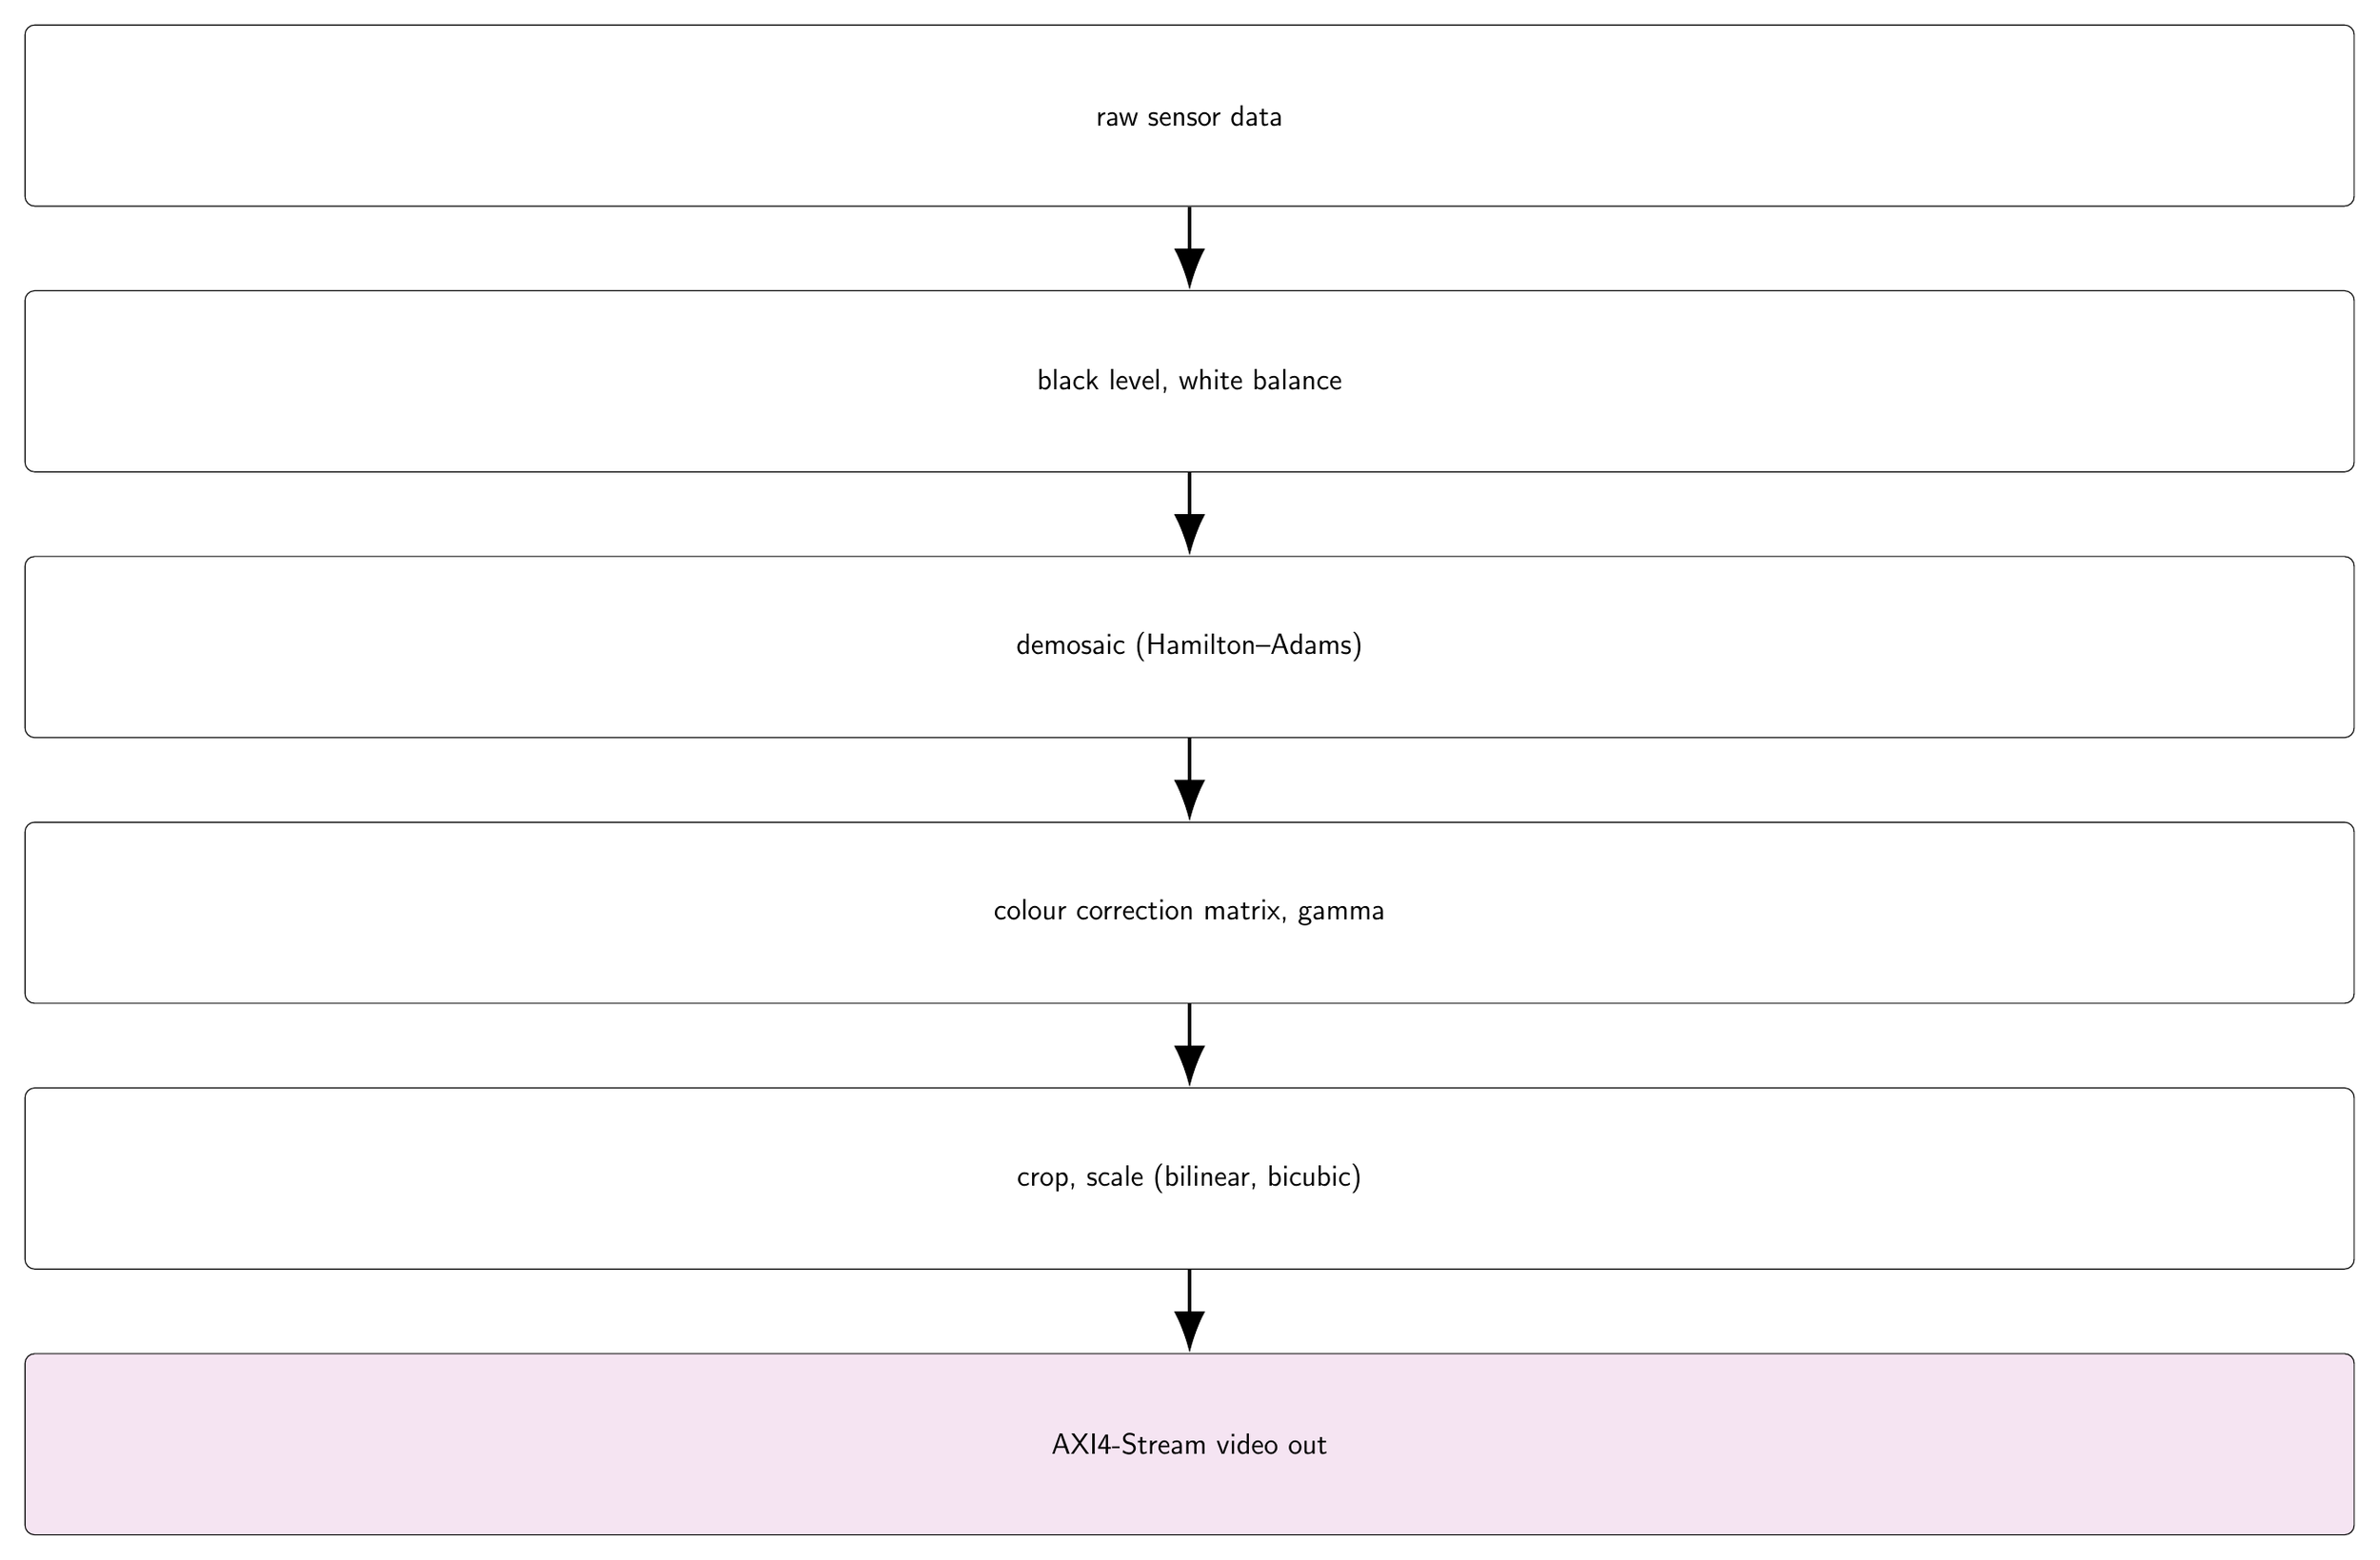
\begin{tikzpicture}
    \node[st] (s) {raw sensor data};
    \node[st, below=12mm of s] (a) {black level, white balance};
    \node[st, below=12mm of a] (b) {demosaic (Hamilton--Adams)};
    \node[st, below=12mm of b] (c) {colour correction matrix, gamma};
    \node[st, below=12mm of c] (d) {crop, scale (bilinear, bicubic)};
    \node[hw, below=12mm of d] (e) {AXI4-Stream video out};
    \foreach \x/\y in {s/a, a/b, b/c, c/d, d/e} \draw[arr] (\x) -- (\y);
  \end{tikzpicture}\\[4mm]
  \raggedright\draft{the order and the blocks to show are Serge's call}
}
\pblock{One model, bit-exact}{
  Each block has one integer model: it is the specification and the reference. The generated
  Verilog is checked against it bit for bit in Verilator and cocotb. Registers over AXI4-Lite,
  described in SystemRDL; a FuseSoC core for integration. Time-of-flight blocks too.
}

\column{0.5}
\pblock{Borg: pixels out}{
  \textbf{A GPU you can read end to end}, in Chisel, with a 64-bit RISC-V CPU that boots Linux,
  a Rust DRM/KMS driver and a native Mesa Vulkan driver in Rust with its own shader compiler.
  \begin{center}\photo{18cm}{the Nexys Video, vkcube full screen over HDMI}\end{center}
  \textbf{Running here:} the unmodified Khronos \texttt{vkcube} under Linux, rendered by Borg.
}
\pblock{How Borg draws a frame}{
  \centering
  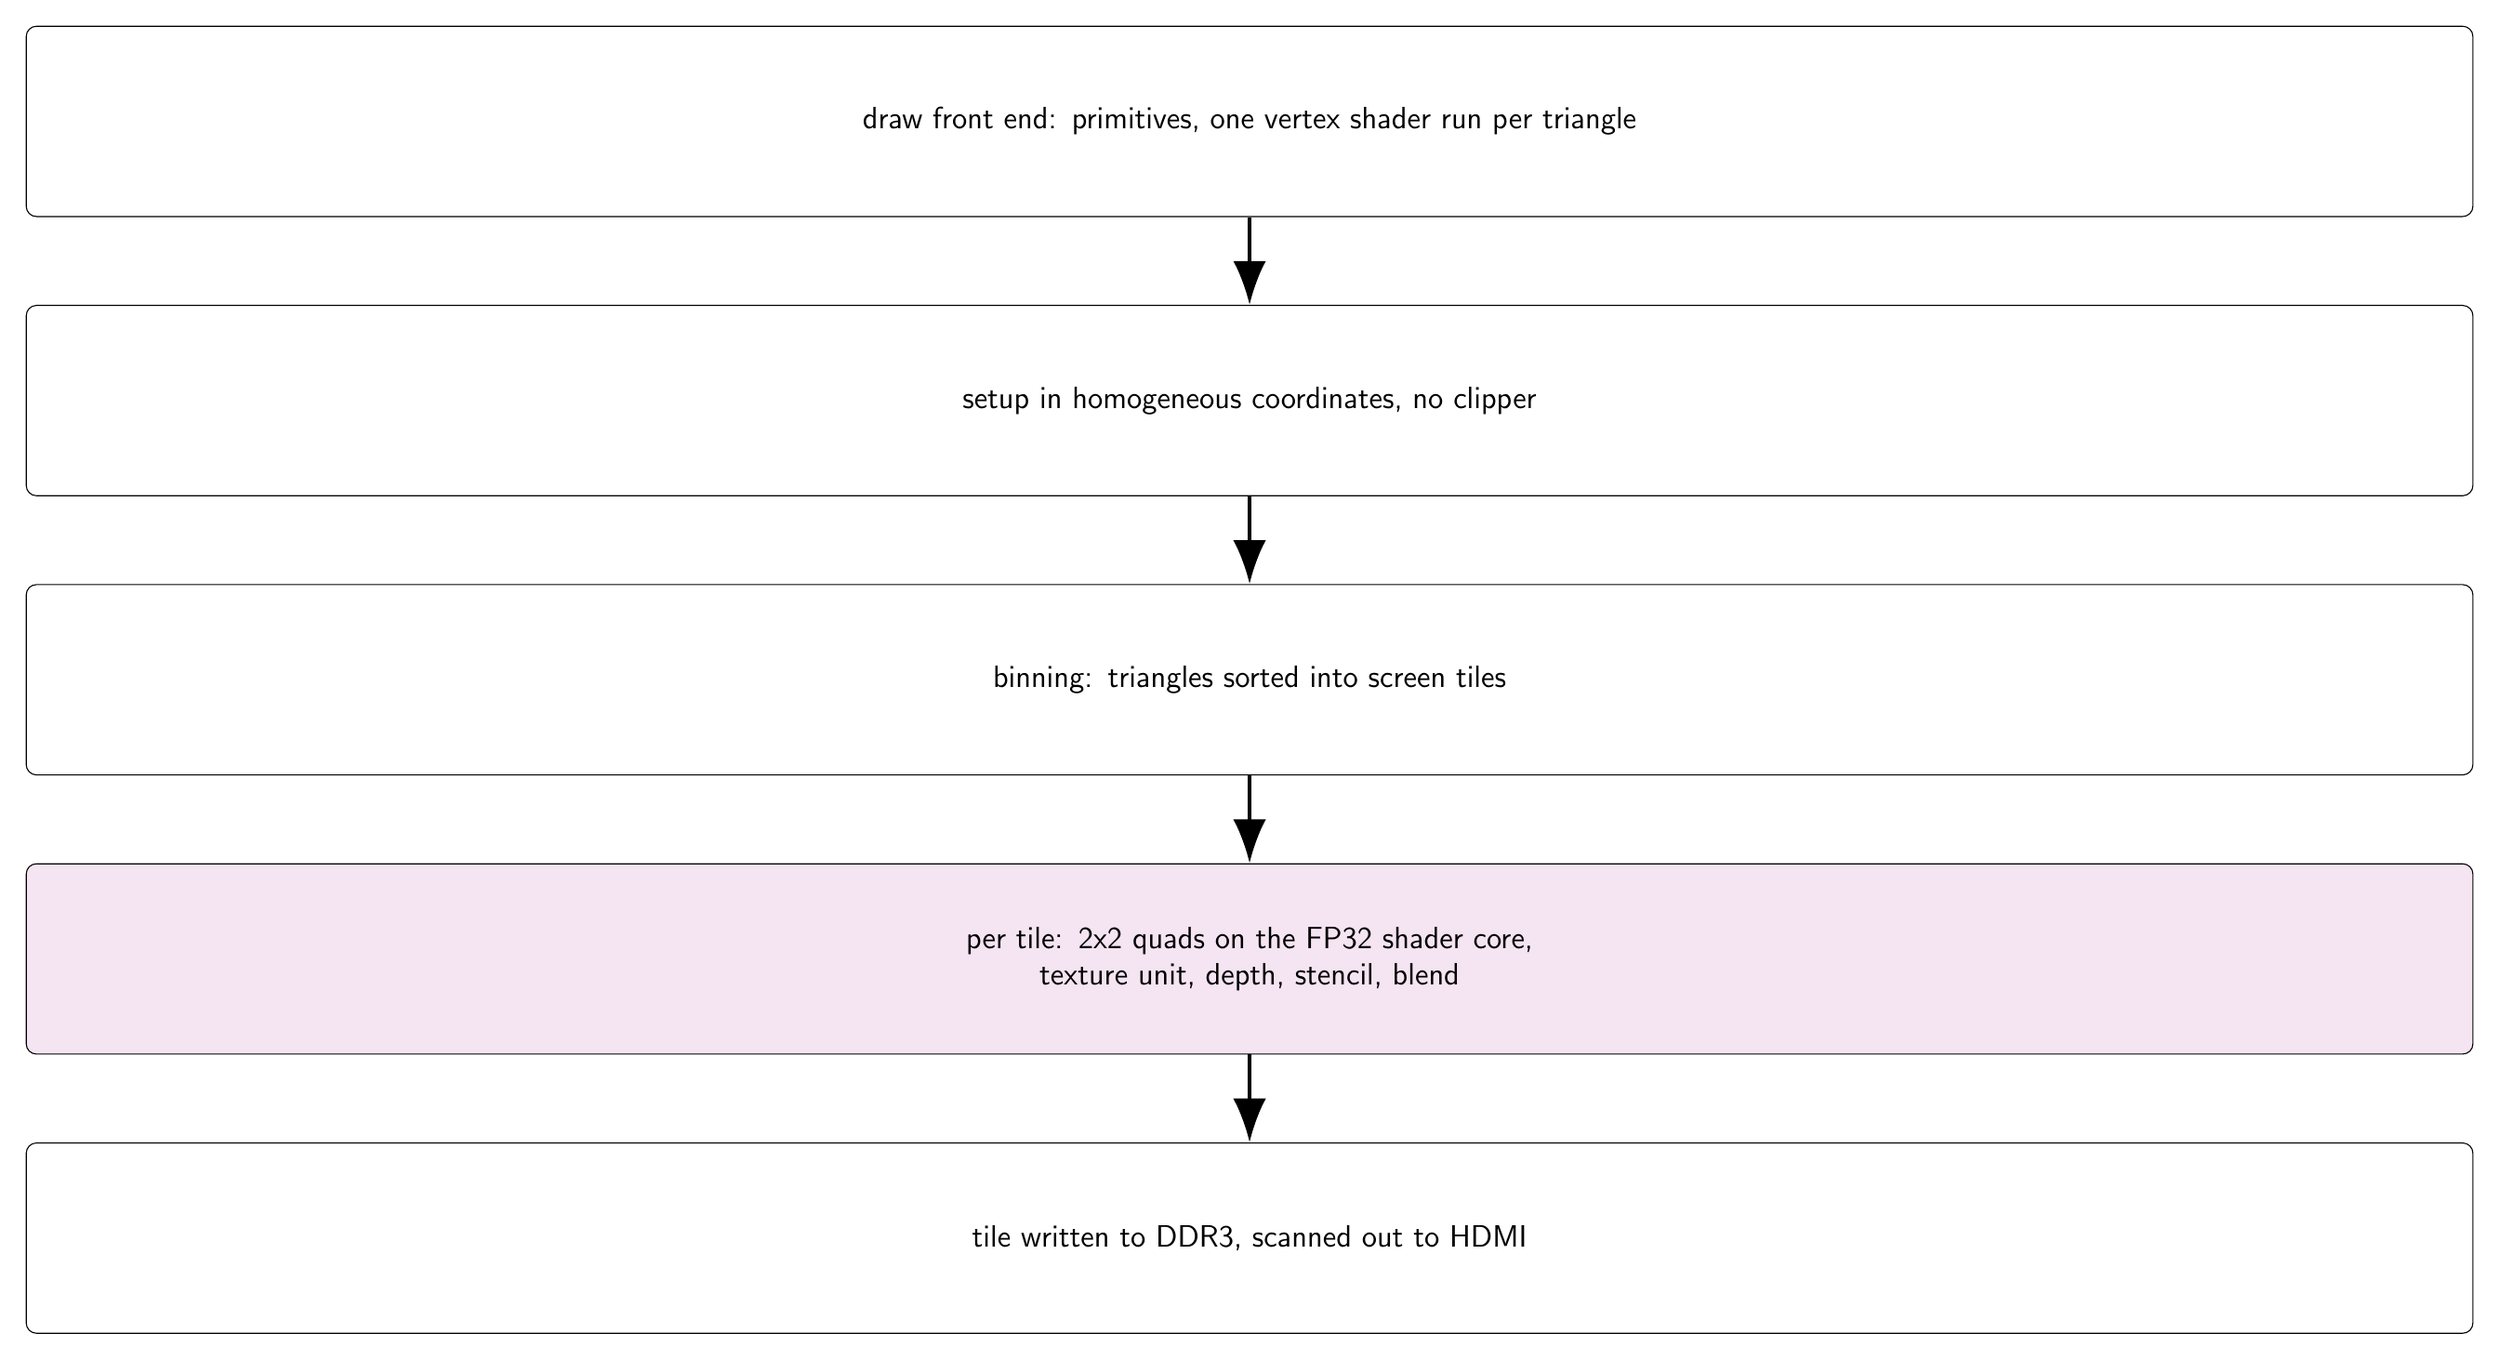
\begin{tikzpicture}
    \node[st] (a) {draw front end: primitives, one vertex shader run per triangle};
    \node[st, below=12mm of a] (b) {setup in homogeneous coordinates, no clipper};
    \node[st, below=12mm of b] (c) {binning: triangles sorted into screen tiles};
    \node[hw, below=12mm of c] (d) {per tile: 2x2 quads on the FP32 shader core,\\texture unit, depth, stencil, blend};
    \node[st, below=12mm of d] (e) {tile written to DDR3, scanned out to HDMI};
    \foreach \x/\y in {a/b, b/c, c/d, d/e} \draw[arr] (\x) -- (\y);
  \end{tikzpicture}
}
\pblock{The whole stack open}{
  \begin{itemize}
    \item Mesa Vulkan driver (borgvk) and shader compiler (borgc) in Rust.
    \item Linux on Hutt, Borg's own RV64 CPU; the DRM/KMS driver in Rust.
    \item The Vulkan conformance tests run on the board, checked byte for byte against a
      simulator of the RTL.
  \end{itemize}
}
\end{columns}

\pblock{What both have in common}{
  \begin{minipage}[c]{0.62\linewidth}
    \begin{itemize}
      \item Hardware generated from a high-level description: NumPy through np2hw, Chisel through CIRCT.
      \item Verified bit for bit against a model, in Verilator and cocotb.
      \item Registers described once, in SystemRDL.
      \item Open source, down to the RTL.
    \end{itemize}
  \end{minipage}\hfill
  \begin{minipage}[c]{0.36\linewidth}
    \centering
    \qrcode[height=8cm]{https://github.com/lanserge/revela}\hspace{3cm}\qrcode[height=8cm]{https://github.com/gonsolo/Borg}\\[3mm]
    revela \hspace{8cm} Borg
  \end{minipage}
}
\end{document}
